 \documentclass[11pt]{article} 
\usepackage[english]{babel}
\usepackage{pgfplots}
\usepackage{polynom}
\usepackage{hyperref}
\pgfplotsset{compat=1.6}

\pgfplotsset{soldot/.style={color=blue,only marks,mark=*}} \pgfplotsset{holdot/.style={color=blue,fill=white,only marks,mark=*}}

\usepackage[utf8]{inputenc}\usepackage{amsmath}
\usepackage{amssymb}
\usepackage{graphicx}
\usepackage[colorinlistoftodos]{todonotes}
\usepackage{listings,multicol}
\setlength{\oddsidemargin}{0.5cm} \setlength{\evensidemargin}{0cm}
\setlength{\textwidth}{16cm} \setlength{\textheight}{23cm}
\setlength{\topmargin}{-0.5cm}
\textheight 21.5cm
\newcommand{\function}[5]{
\begin{array}{cccl}
#1 :& #2 	& \longrightarrow 	& #3\\
	& #4	& \longmapsto		& #5
\end{array}
}

\usepackage[numbered,framed]{matlab-prettifier}
\lstMakeShortInline"
\lstset{
  style              = Matlab-editor,
  %basicstyle         = \mlttfamily,
  escapechar         = ",
  mlshowsectionrules = true,
}

\begin{document}

\title{T2 V1 NUMERICO 521230 UDEC}

\begin{minipage}{0.12\textwidth}

\includegraphics[width=\textwidth]{logoudec.eps}
\end{minipage}
\hspace{5mm}
\begin{minipage}{0.9\textwidth}
UNIVERSIDAD DE CONCEPCION\\
{\small\small\bf 
FACULTAD DE CIENCIAS\\ 
FISICAS Y MATEMATICAS}\\
DEPARTAMENTO DE INGENIERIA MATEMATICA\\
\rule{0.66\textwidth}{.5pt} Franco A. Milanese
\end{minipage}

\vspace{0.5cm}
\centerline{\bf Test II (521230)}
\begin{center}
 \begin{tabular}{p{0.7\textwidth}p{0.3\textwidth}}
	\textbf{Nombre:}   &\textbf{Carrera:}\\
	\textbf{Profesor:} & \textbf{ RUT:}
 \end{tabular}
 \\
 \vspace{0.2cm}
 \begin{tabular}{||p{2cm}|p{2cm}||p{2cm}||}
 \hline
 Pregunta 1 &  Pregunta 2 &     Total\\
 \hline

  \vspace{1.5cm} & &       \\
 \hline
 \end{tabular}
 \end{center}
 Enviar documentos solicitados en el formato solicitado a 
 %\textbf{veranonumerico@gmail.com}.

\begin{enumerate}
\item (30 pt) Sean las funciones
$$
f(x)=\frac{sin(\pi x)}{x^2+1},
\quad
g(x)=f(x+1).
$$
En un rutero llamado \texttt{p1v1.m} estime, usando la regla del punto medio, y en una partici\'on uniforme de tamaño $10^{-3}$ 
    $$
    \int_0^{10} f(x)dx, \quad 
        \int_0^{10} g(x)dx. 
    $$
\textbf{Desarollo:} Debe tener un c\'odigo similar a \fbox{30pt}
\begin{lstlisting}
f=@(x) sin(pi*x)./(x.^2+1);
h=10^(-3);
node=[0:h:10]+1/2*h;
int1=sum(f(node))*h
int2=sum(f(node+1))*h
\end{lstlisting}
y los valores aproximados calculados son 
\begin{lstlisting}
int1 =

    0.3592


int2 =

   -0.1395

\end{lstlisting}

\item (30 pt) En un rutero llamado \texttt{p2v1.m}
\begin{enumerate}
\item Grafique la funci\'on 
$$
j(x)=\frac{cos(\pi x)}{e^{x^2+2x+1}},
$$
en el intervalo $[-10,0]$.
\item Programe el m\'etodo de la bisecci\'on para que calcule la ra\'iz de de la funci\'on que se encuentra a la derecha de $x=-2$, con una tolerancia de $10^{-8}$.
\end{enumerate}
\textbf{Desarollo:}
El rutero debe tener las instrucciones
\begin{lstlisting}
clear all; close all; clc;
j=@(x) cos(pi*x)./exp(x.^2+2*x+1);
plot(-10:0.01:0,j(-10:0.01:0)); grid on; hold on;
x0=-2;
x1=-1;
tol=1;
while tol>10^(-8)
   x2=(x0+x1)/2;
   tol=abs(j(x2));
   if(j(x0)*j(x2)<0)
       x1=x2;
   else
       x0=x2;
   end
end
format long
x2;
\end{lstlisting}
\begin{enumerate}
\item La gr\'afica debe ser de la forma

\begin{centering}
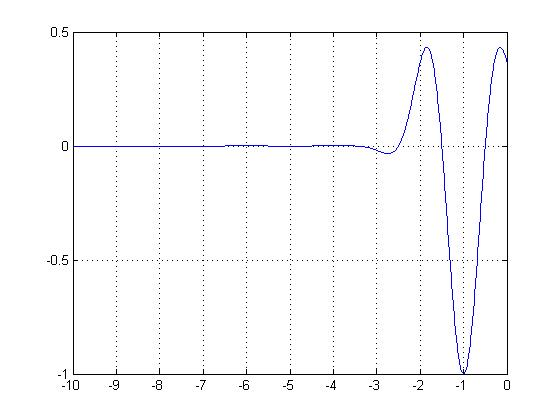
\includegraphics[width=0.7\textwidth]{./p2v1.jpg}
\end{centering}
\item 
\begin{lstlisting}
x2 =

  -1.500000000000000

\end{lstlisting}
\end{enumerate}
\end{enumerate}
\end{document}  